%" vim: fdm=marker:fen:fdl=0
% Manufacturing of Planar Detectors Chapter intro%{{{
\chapter{Manufacturing of Planar Detectors}
The manufacturing process of a planar HPGe detector begins with a slice from a crystal boule that has been tested for quality and is know to be detector grade.
Typical boules slices are solid discs that can range from a few millimeters up to several centimeters in thickness and 5+ centimeters in diameter.
This large size allows for several detector samples to be cut from each slice so careful geometry considerations are important in order to minimize wasted material.
The goal is for the detector sample to look approximately like figure \ref{fig:dummydet} which is an example of a planar detector with so called top hat geometry.
\begin{figure}[htpb]
\centering
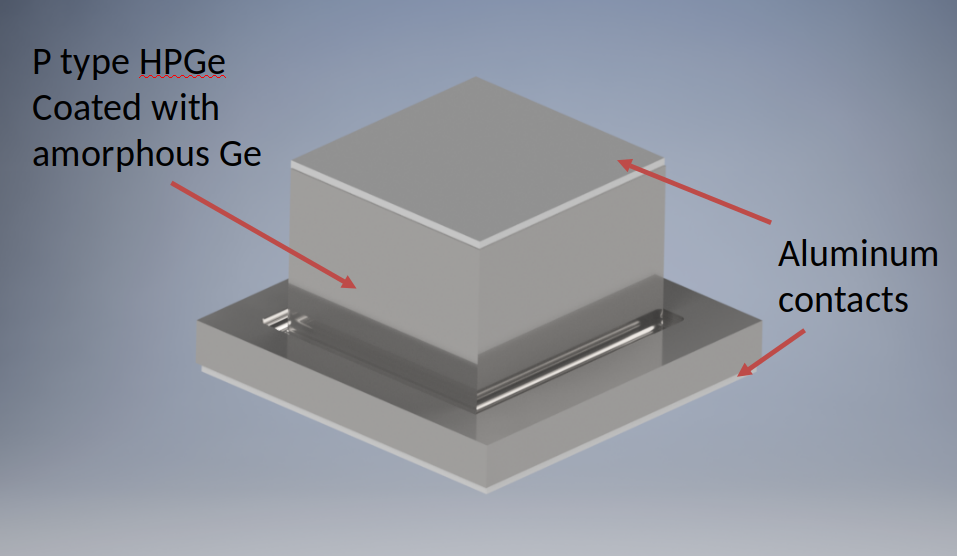
\includegraphics[width=0.5\textwidth]{dummy-det}
\caption{Example detector geometry with four wings}
\label{fig:dummydet}
\end{figure}
The brims of the hat are called wings and serve as a dead area of the detector for handling during the manufacturing process.
The detector is not required to be perfectly square to work so length and width can vary within a few centimeters.
What is of importance are the overall thickness and that the top and bottom faces are parallel.
Due to the relatively long mean free path of gamma rays in germanium, a detector should aim to be at least one centimeter thick.

Once considerations for geometry have been made, the detector manufacturing process begins.
To start, the germanium boule slice is cut into several rectangular cubes.
Then, work proceeds using one of the cubes, saving the rest for the next time.%}}}
% Section: Mechanical Processing%{{{
\section{Mechanical Processing}
The diamond saw under discussion is the SYJ-400 Precision CNC Dicing/Cutting Saw from Shenyang Kejing Auto-Instrument Co.
The structure of this diamond saw is shown below in Figure \ref{fig:diamondsaw}.
It is operated using a CNC controller with setting for the cutting speed, length, time, depth, lifting height, rest time, and movement speed.
All of these parameters are edited using the attached CNC controller. 
There are four separate screens with adjustable parameters that are shown with translations in Figure \ref{fig:control-screen}. 
Each of these parameters are in millimeters or millimeters per minute depending on the operation.
\begin{figure}[htpb]
\centering
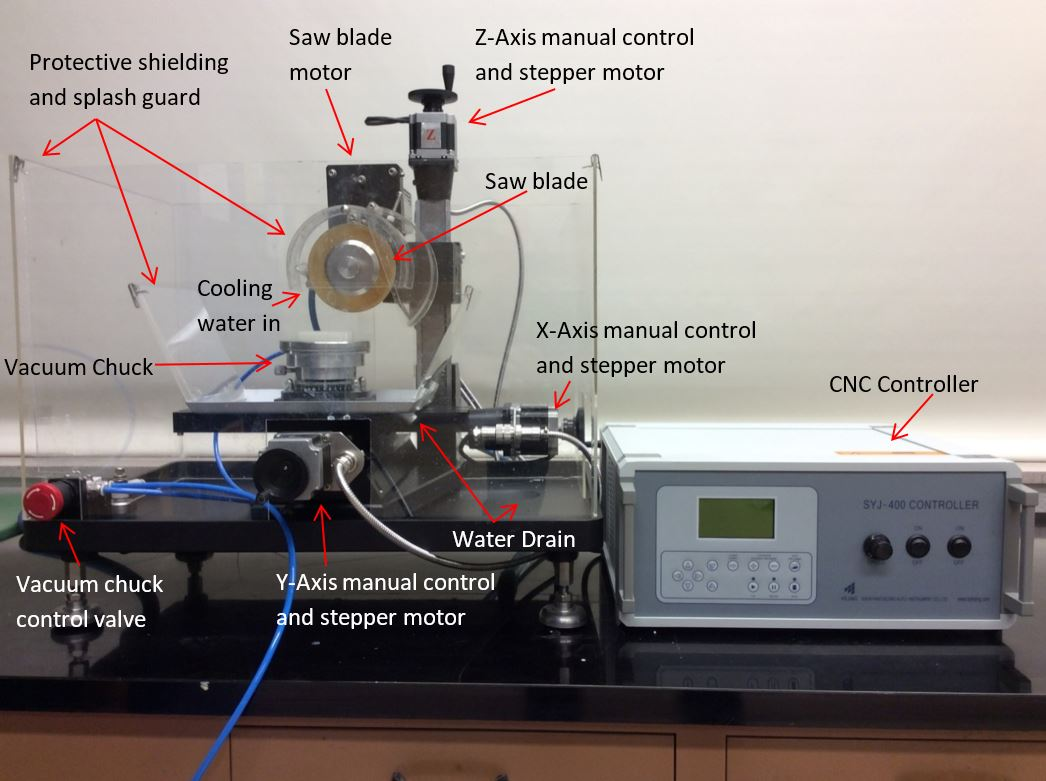
\includegraphics[width=0.8\textwidth]{diamond-saw.jpg}
\caption{The diamond saw used to cut boules into detector samples.}
\label{fig:diamondsaw}
\end{figure}

Before turning on the power to the diamond saw, it is important to take care of all of the necessary adjustments such as changing blades and placing the sample onto the vacuum chuck.
It is important to do this before supplying power in order to prevent the saw from somehow starting itself.
To switch blades, first remove the finger screw, labeled 1, on the outside of the splash guard covering the blade. Then remove the finger screw, labeled 2, that holds the blade clamps.
Remove the outer blade clamp and the blade can be switched out.
Depending on the blade size, it may be necessary to change to a larger splash guard.
To do this, first remove finger screw 1 on the outside of the splash guard, then remove the two hex screws, labeled H, on the back plate.
It might be necessary to remove the blade to access these screws.
You can then install the new splash guard and blade working in the opposite order to put everything back together.
\begin{figure}[htpb]
\centering
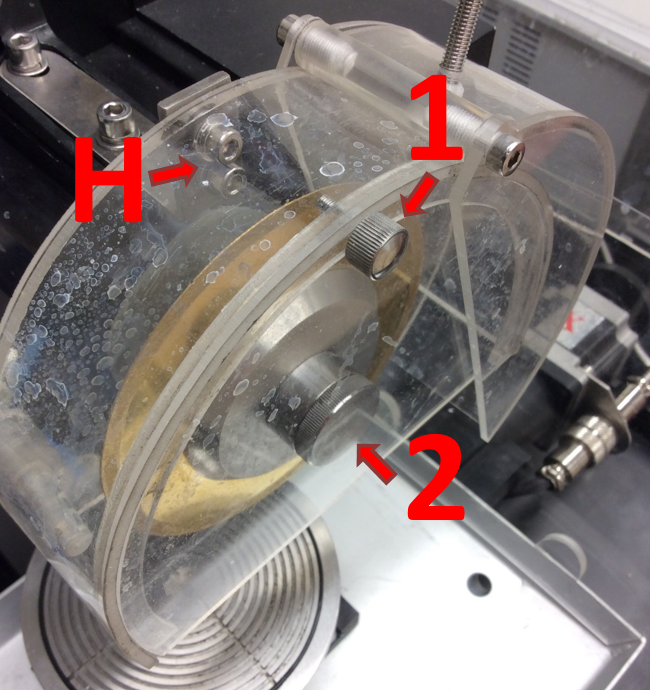
\includegraphics[width=0.5\textwidth]{blade-case.PNG}
\caption{This is the blade and shielding on the diamond saw.}
\label{fig:blade-case}
\end{figure}

There are currently three different blades available for cutting.
They are all four inches in diameter and include: an electroplated diamond blade, full sintered diamond blade, and a 2mm grinding wheel.
The electroplated blade is thin and useful for the initial cuts of the boule.
The grinding wheel is used to make grooves and grind down the detector wings.
\begin{figure}[htpb]
\centering
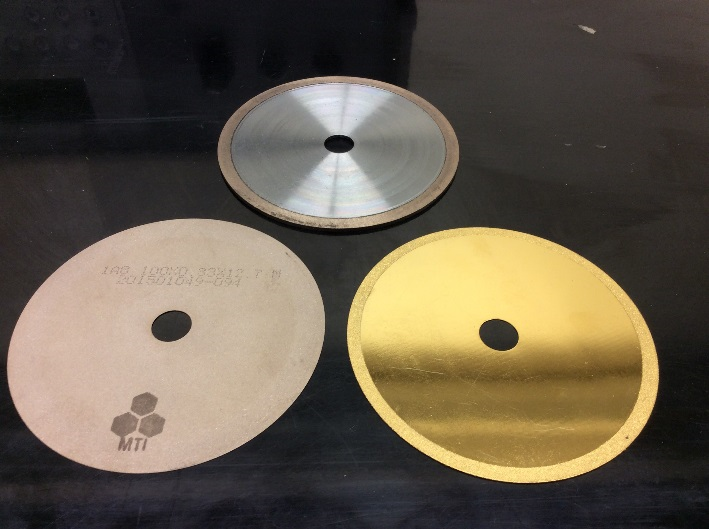
\includegraphics[width=0.5\textwidth]{blades}
\caption{Three different blade types for cutting germanium.}
\label{fig:blades}
\end{figure}

The next step is to mount your sample onto the vacuum chuck.
It is essential to do this before powering on the diamond saw to avoid accidents.
Place the steel sample holder onto the vacuum chuck and adjust it so it is properly aligned.
The vacuum can then be turned on to suction the chuck and keep the sample from moving during cutting.
To start the diamond saw, the power strip must be plugged in and turned on.
The strip will provide power to the vacuum pump and the up/down voltage converter.
The next step is to power on the up/down converter that is located under the table that supports the diamond saw.
The converter will provide a stepped up voltage to the CNC controller (which powers the saw) and the water pump.
The saw controller requires 220 volts which is why it cannot be plugged into a standard outlet.

The first cuts of the boule should be made with the thin diamond blade and go all the way through the germanium into the graphite plate.
The initial cuts are to cut the rough detector shape out of the crystal slice.
An example of a cut boule can be seen in Figure ~\ref{fig:cutboule} where four detector samples are cut from a single crystal.
\begin{figure}[htpb]
\centering
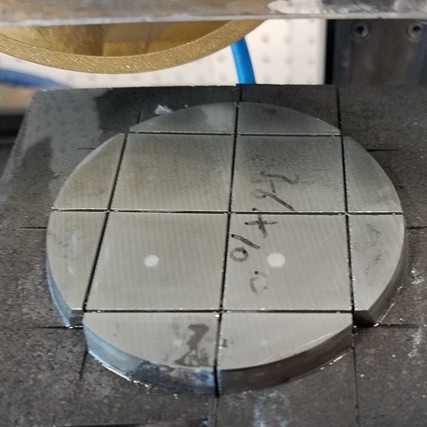
\includegraphics[width=0.5\textwidth]{cut-boule.jpg}
\caption{This is the crystal boule after the initial detector sample blanks have been cut.}
\label{fig:cutboule}
\end{figure}
The saw must be start and stopped using the provided controller.
All of the settings and translations can be seen in the appendix in Figure ~\ref{fig:control-screen}.
One property of germanium is that it is an extremely brittle metal.
This can cause problems when cutting because the material will chip under normal cutting speeds.
Due to this problem, the diamond saw must travel less that a millimeter per minute and grind the germanium instead of cutting it.

After the detector blanks have been cut from the boule, the stainless steel and graphite plate are reheated to melt the wax and remove all the extra pieces.
A single detector sample is then left and centered on the graphite for further cutting.
The next step is to replace the thin blade with the grinding wheel so that the groove cuts can be made.
A detector can have either two or four wings depending on the final goal.
The groove are ground out approximately two millimeters from the edge of the sample, then the sample is moved and the remaining bits are ground down to leave the wing shape.
An example of a detector with four wings is shown in Figure ~\ref{fig:cut-sample}.
\begin{figure}[htpb]
\centering
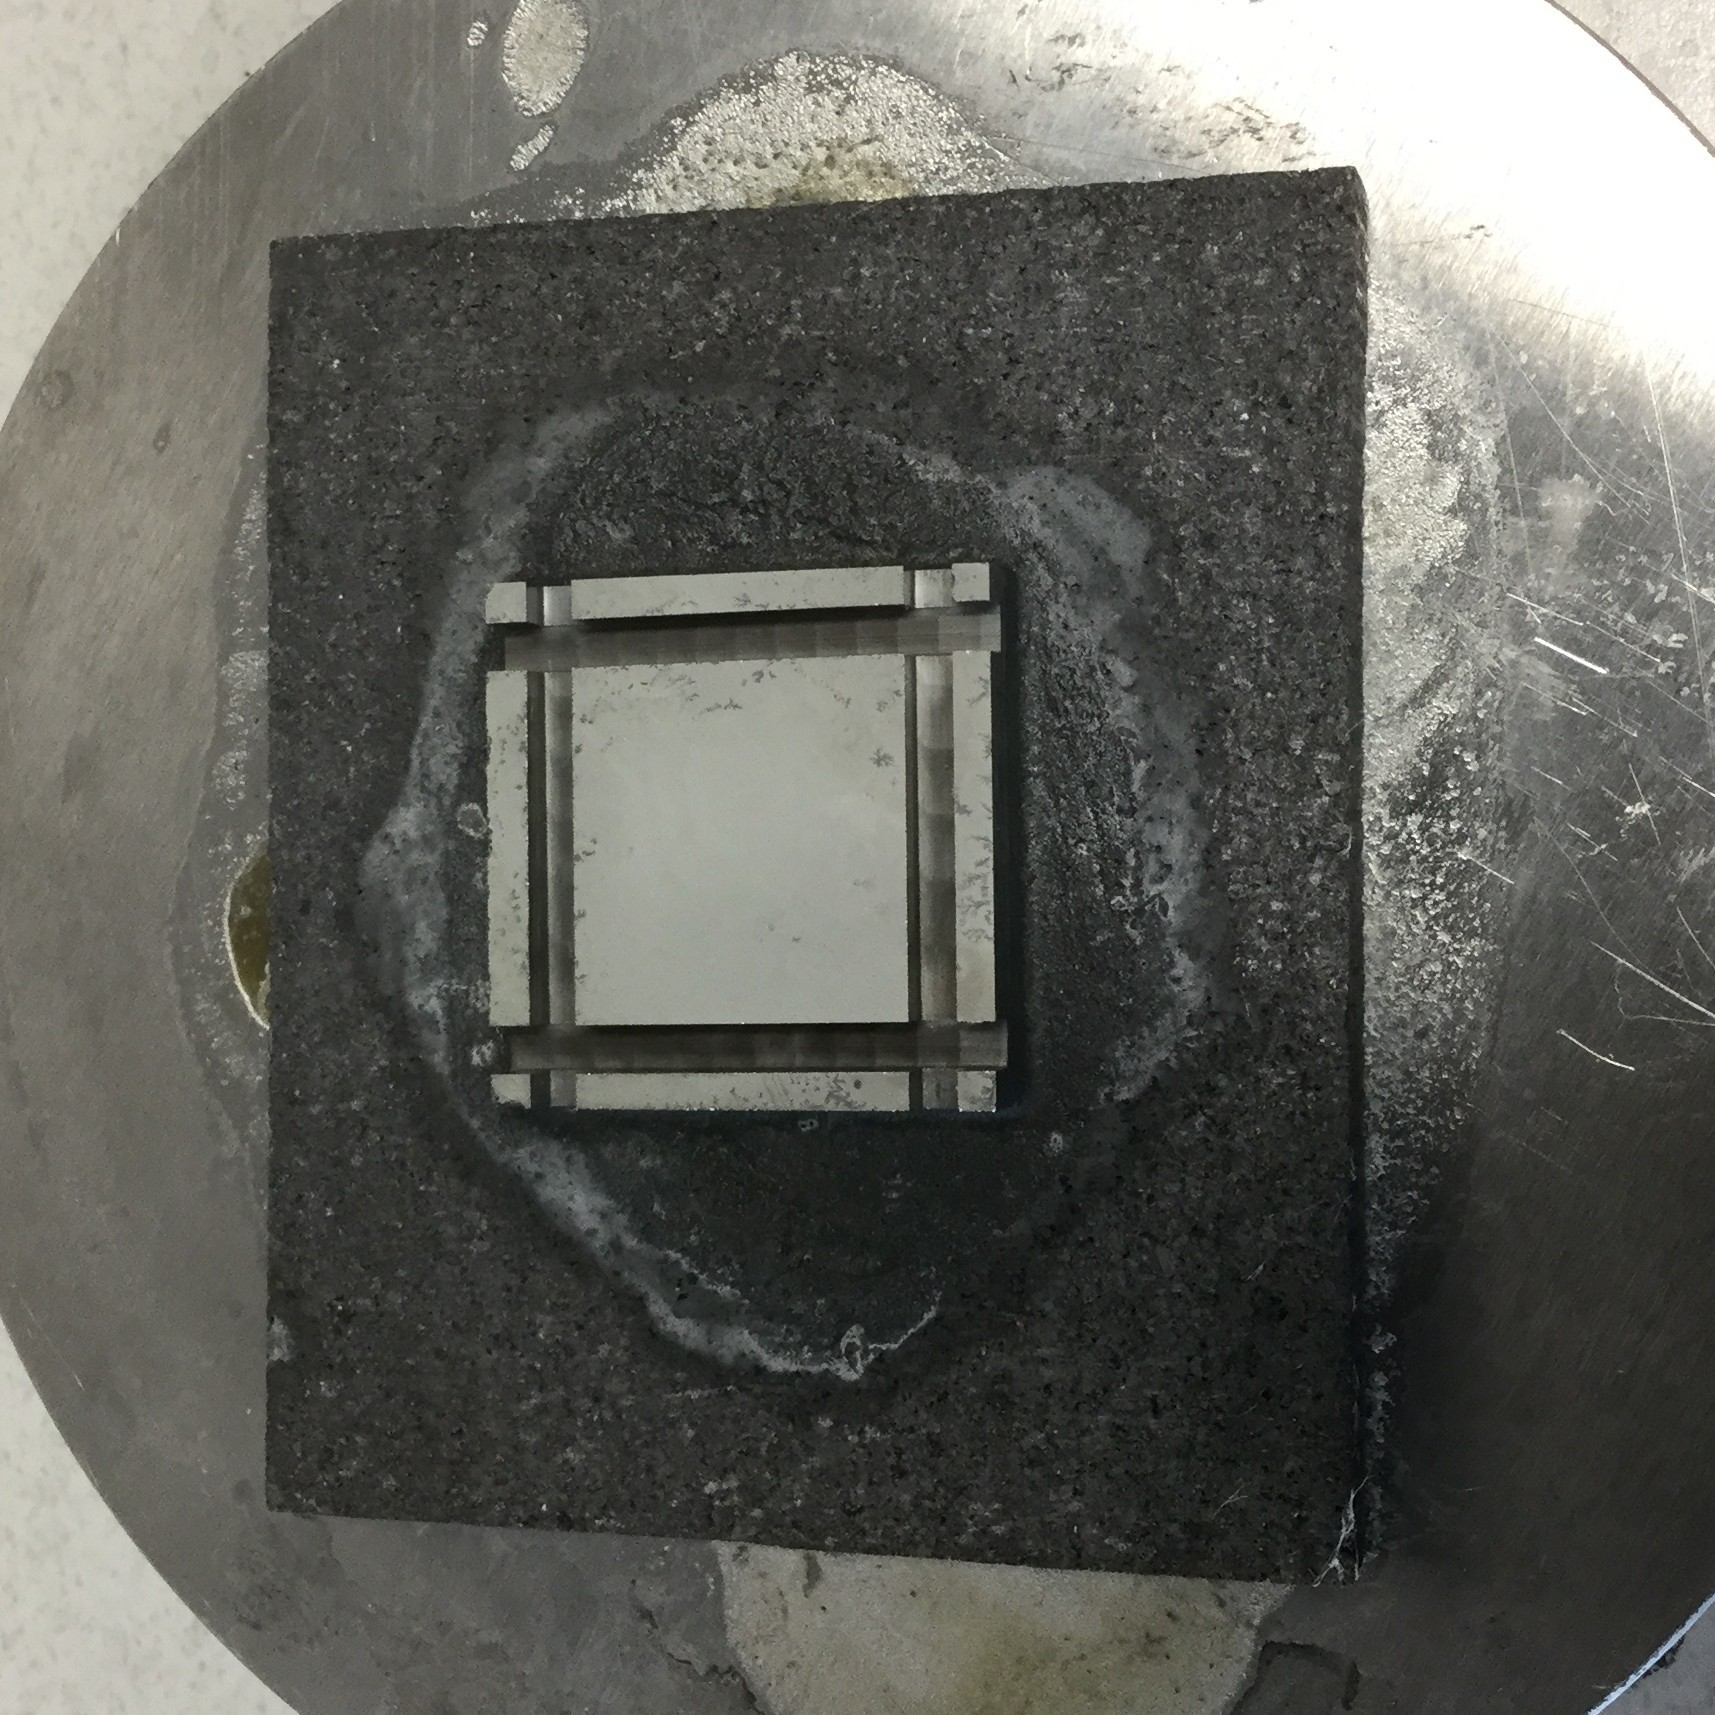
\includegraphics[width=0.5\textwidth]{cut-sample.JPG}
\caption{A germanium sample mounted on graphite which is then mounted on a stainless steel chuck.}
\label{fig:cut-sample}
\end{figure}

After the detector has finished up in the diamond saw, it is left with a very rough surface that might have some minor chipping along the edge.
Any cracks or large chips can lead to detector failure down the line so they must be removed before continuing.
The first and most effective way to remove material is through lapping.
For lapping, an abrasive is mixed with water on a glass plate or polishing pad to create a slurry.
Figure \ref{fig:lapping} shows the glass plate with polishing pad on top along with a detector sitting in the slurry.
The detector is then ran across the slurry which slow grinds down the surface.
The speed of material removal is based on the type and particle size of the abrasive.
Two types of abrasives are used for lapping at USD, one is silicon carbide (SiC) and the other is aluminum oxide (Al$_2$O$_3$).
To remove lots of material, the larger grit SiC is used.
The brand ID is Lapmaster 2600 and it has an average particle size of 17.5 micron.
For finer polishing the aluminum oxide with average particle size of 9.5 micron is used.
There 9.5 micron is called Lapmaster 1900.
The Al$_2$O$_3$ is available in several particle sizes where the most used at USD are the 9.5 micron and 1 micron versions.
\begin{figure}[htpb]
\centering
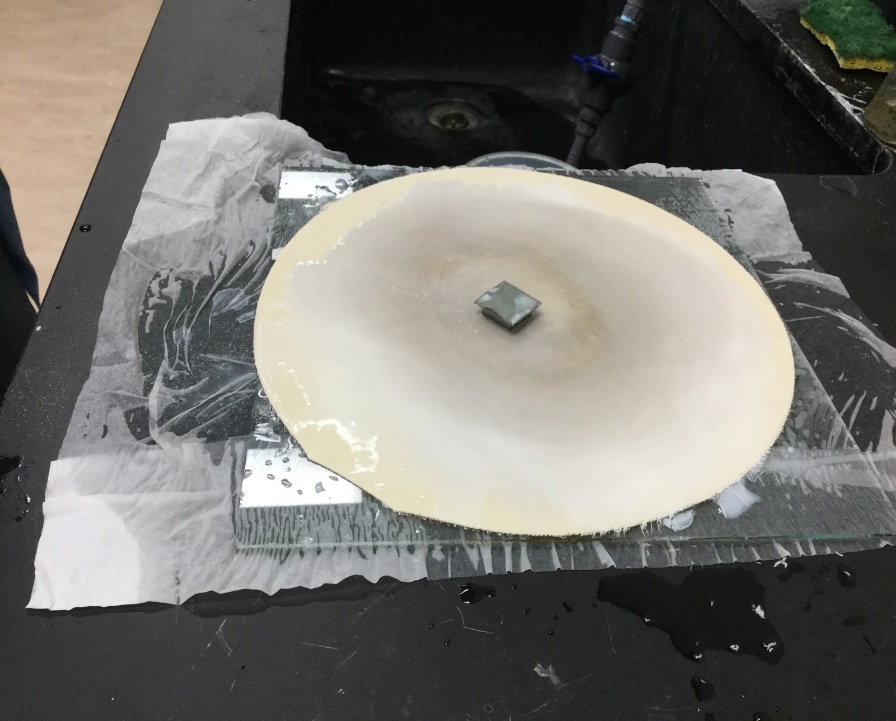
\includegraphics[width=0.5\textwidth]{lapping.jpg}
\caption{An example of lapping the detector sample}
\label{fig:lapping}
\end{figure}
Generaly the 9.5 micron Al$_2$O$_3$ is enough to remove major defects from the diamond saw and perpare for chemical polishing.
The standard procedure is to spoon out a few grams of the abrasive onto the glass slide.
Then enough DI water to create a slurry is mixed into the powder.
The detector is then slid around on the slurry which slowly polishes the surface.
Ocassionaly further polishing is required to reduce the amount of time required for chemical processing.
In order to achieve a mirror like finish prior to acid etching, a polishing pad can be used.
When using the polishing pad, shown in Figure \ref{fig:lapping}, it is important to use an abrasive of 3 microns or less to achieve a nice finish.
%}}}
% Section: Chemical Processing%{{{
\section{Chemical Processing}

The cutting and lapping leaves the surface of the detector with micro scratches and defects, sometimes invisible to the naked eye, that could lead to failure down the process line if not treated properly.
Since the next step of detector fabrication involves depositing thin layers of metal that need to stick together, it is important that the surface is as smooth and clean as possible.
Acid etching is a useful tool to remove the outer layer of germanium and leave behind a smooth and defect free surface as long as the right chemical mixture is used.  

Several chemical treatments are commonly used in the semiconductor industry to deal with such cleaning and polishing.
For cleaning there are solvents such as acetone, methanol, and Trichloroethylene that are used to remove the wax and debree after cutting.
The detector manufacturing lab is equipped with a metal hood for such operations involving these solvents that is shown in Figure ~\ref{fig:metalhood}
\begin{figure}[htpb]
\centering
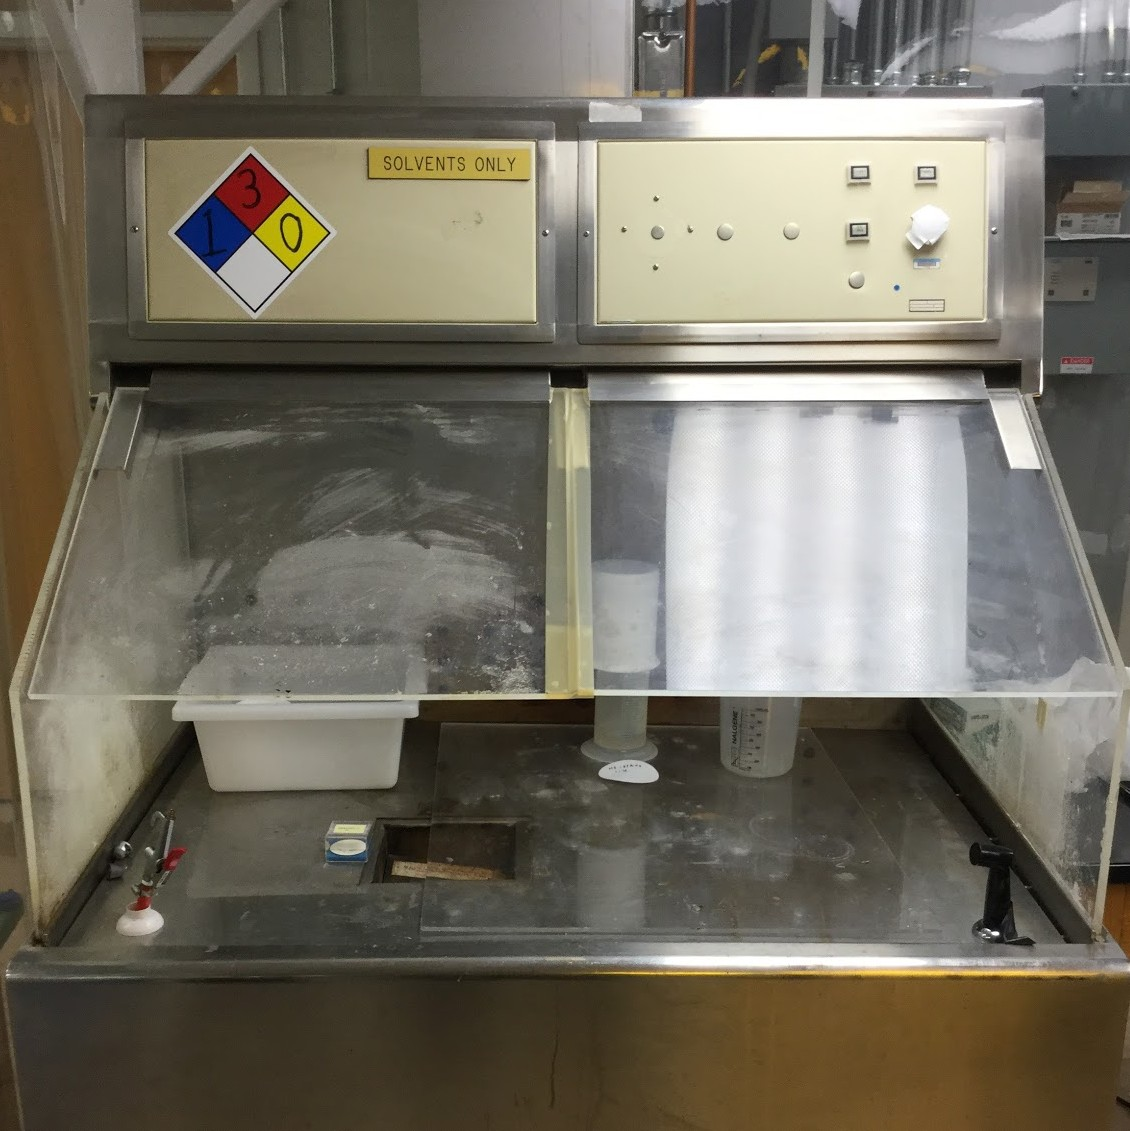
\includegraphics[width=0.5\textwidth]{metal-hood.jpg}
\caption{Metal hood for use with solvents}
\label{fig:metalhood}
\end{figure}

For polishing it is standard to use an acid etch, usually a mixture of Nitric (HNO$_3$) and hydrofluoric (HF) acids.
The ratio of the two acides will determine how agressive the etch is.
For detector fabrication a 4:1 HNO$_3$:HF ratio is used.
Figure \ref{fig:plastichood} shows the plastic hood that is used for acid etching.
\begin{figure}[htpb]
\centering
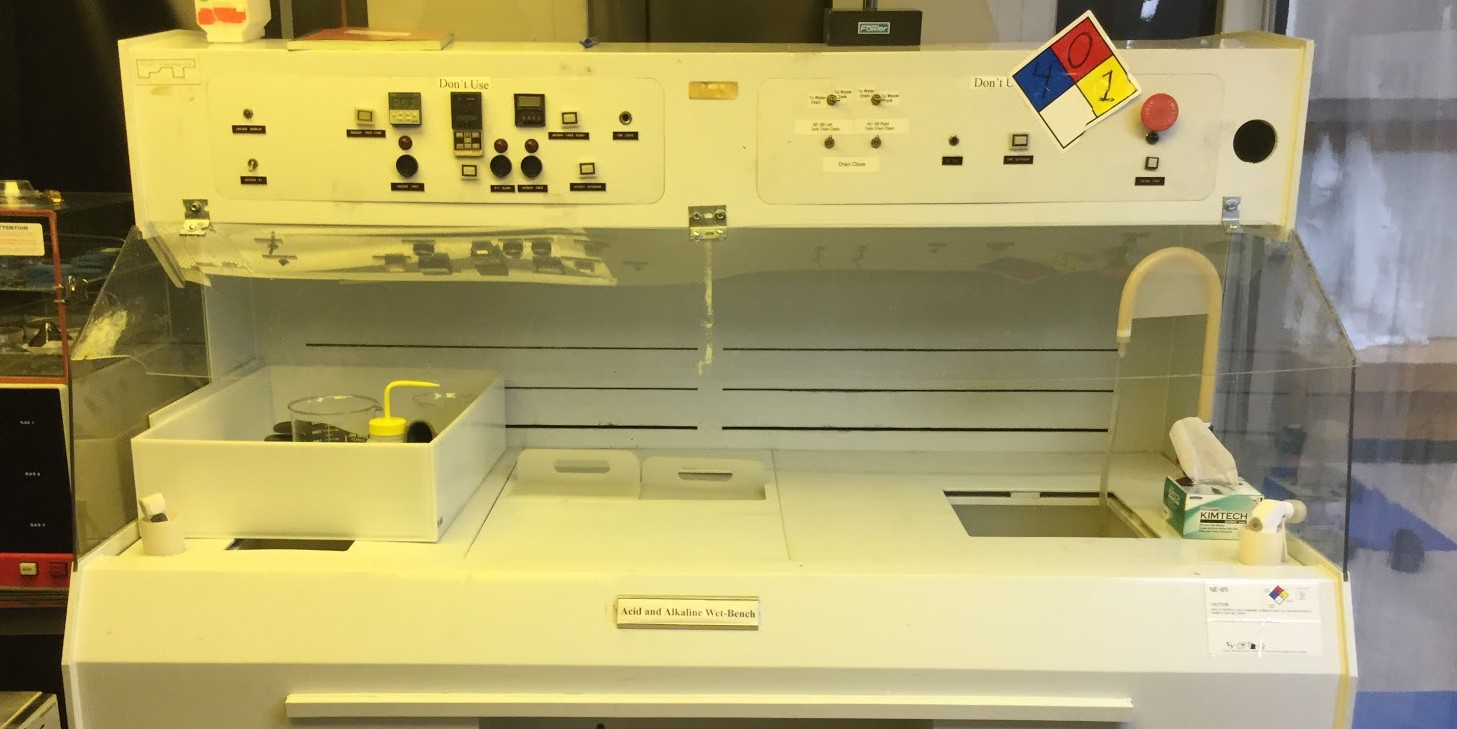
\includegraphics[width=0.7\textwidth]{plastic-hood.jpg}
\caption{Plastic hood for use with acids.}
\label{fig:plastichood}
\end{figure}
To prepare for sputtering and aluminum deposition, two etches are required.
Both etches are in the 4:1 solution, however, the time varies.
The first etch is around three minutes long and takes place after lapping.
This longer etch is meant to fully polish the crystal and rid it of scratches and defects.
The second etch is only 30 seconds and is to clean the surface of the crystal immediately before it is loaded into the sputtering machine.

The procedure for acid etching starts with taking proper precautions to ensure safety and prevent accidents.
Heavy duty gloves are worn overtop several layers of lab gloves, along with safety goggles, lab coat, and respirator if necessary.
Then the acid mixture can be made.
Figure \ref{fig:acidbeakers} shows the acid bottles along with several beakers and a graduated cylinder.
The graduated cylinder is used to measure out the proper ratio of acids, usually 160 ml of nitric acid is poured in first followed by 40 ml of hydrofluoric.
This is enough solution for at least two etches.
Approximately 100 ml of solution is then poured into an empty PTFE beaker.
It is also necessary to have at least three beakers filled with DI water, two for quenching after the etch and one two quench any paper waste.
\begin{figure}[htpb]
\centering
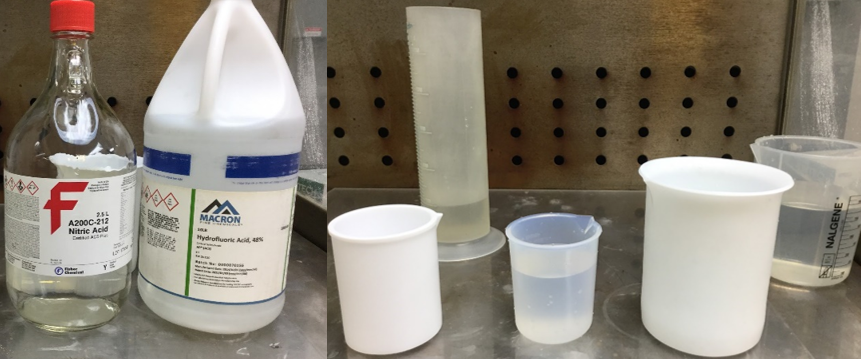
\includegraphics[width=\textwidth]{acidbeakers}
\caption{Left: Nitric and Hydrofluoric acid bottles. Right: Graduated cylinder PTFE and plastic beakers}
\label{fig:acidbeakers}
\end{figure}
After the setup is complete, etching can proceed.
For the longer three minute polish, the clean detector sample is placed in the acid using longacid resistant tweezers.
The detector must then be continuously agitated and flipped halfway through to ensure a uniform etch.
After the three minutes have elapsed the detector is removed and immediately dipped into the first DI water beaker for a few seconds to stop the etch.
Then it is dipped into the second DI water beaker to remove any remaining acid.
After the DI water quench, the detector is quickly dried with dry nitrogen to remove all moisture from the surface.
The surface of the detector sample should now have a mirror finish, although some minor cloudiness sometimes arises and is acceptable.
If scratches remain, the detector can be etched further, usually for a minute or less.
\begin{figure}[htpb]
\centering
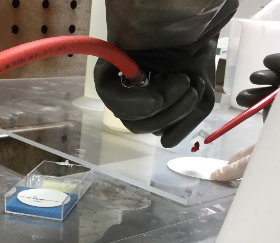
\includegraphics[width=0.5\textwidth]{drynitrogen}
\caption{A detector sample being held and dried with nitrogen.}
\label{fig:drynitrogen}
\end{figure}

At this point the detector sample is ready for the final 30 second etch and loading into the sputtering machine.
The same etch mixture is used as in the long etch, only this time the sample is held continuosly by the tweezers and is swished around in the acid.
Being held continuously prevents the surface from contacting anything other than acid and keeps it free from the possibility that more scratches are introduced.
The steps of quenching in DI water and drying with nitrogen are the same with importance being placed on the sample being held and never allowed to touch any surfaces.
After the detector sample is dried, it can be placed onto the sputtering jig and loaded into the sputtering machine.
%}}}
% Section : Amorphous Ge Deposition%{{{
\section{Amorphous Ge Deposition}

Need information on the working principles of sputtering machine
also need more on the range measurement, marks papers citing specific values for settings 
\subsection{Principles of Sputtering}

\subsection{Operating Procedure}
The sputtering machine at USD is a Perkin-Elmer 4400 Sputtering System.

The operating procedure for the sputtering machine is complex and care is required to make sure the system maintains working order.
It is a complex system with multiple valves, controls, power supplies, vacuum systems, and pressure monitors that all work in conjunction to deposit a thin layer of amorphous germanium on the detector sample.
One key component of the system is a cryopump that uses pressurized helium gas to quickly vacuum the system to the proper pressure.
The cryopump system can be seen in Figure ~\ref{fig:sput-flow} as blue boxes with labels connected by green lines.
The green lines exchange the helium between the cold head connected to the vacuum chamber and the compressor located in the pump room.
Before the sputtering procedure can begin, the cryopump must be turned on to allow the cold head to cool from room temperature to approximately 20K.
Prior to cooling down the cryopump, it must be vacuumed to below 100 mtorr using the rough pump describe later.
In order to vacuum the cryopump, open the forline valve shown as E in ~\ref{fig:sput-flow}; close the valve before turning on the cryopump.
The on/off switch for the compressor is located on the panel with the other valve toggles and is labeled as "HY-VAC PUMP"

Once the cryopump is cooled down to the proper temperature, the sputtering procedure can begin.
As seen in Figure ~\ref{fig:sput-flow}, there are multiple valves for opening and closing various gas and vacuum lines.
These valves are all pneumatically opened and closed so they require a constant supply of pressurized air at 60 psi.
This pressurized air is supplied by a large Kaeser SX 5 compressor located in the pump room and shown in Figure ~\ref{fig:comp-air}.
\begin{figure}[htpb]
\centering
\includegraphics[width=\textwidth]{comp-air}
\caption{Kaeser SX 5 compressor}
\label{fig:comp-air}
\end{figure}
The compressor is turned on or off by pressing the green or red button on the control interface shown on the top left side of the figure.
Once turned on, it will automatically increase in pressure until it reaches a set point around 100 psi.
The pressure out is then reduced or increased by adjusting the pressure regulator shown on the bottom left.
It is important to check the pressure often to make sure that it is sufficiently high for if it drops too low, valves will return to the default closed position.

Once the system has been supplied with pressurized air, the valves can be opened or closed and the system is ready to be operated.
The next step is to load the detector sample into the sputtering machine and prepare for deposition.
The sputtering system should always be kept under vacuum so before it can be opened it must be returned to standard atmospheric pressure.
This is done by opening the vent valve and filling the chamber with dry nitrogen.
The toggle switch for the vent valve is located at 'A' in Figure ~\ref{fig:sput-flow}.
The nitrogen in routed in from a tank located in a separate room behind the pump room and is kept at approximately 10 to 15 psi.

After the chamber has returned to atmospheric pressure it can be opened using a hydraulic lift system that is powered through the RF power generator.
The sample can now be carefully placed inside the chamber centering it under the amorphous germanium target as seen in Figure ~\ref{fig:sput-open}.
\begin{figure}[htpb]
\centering
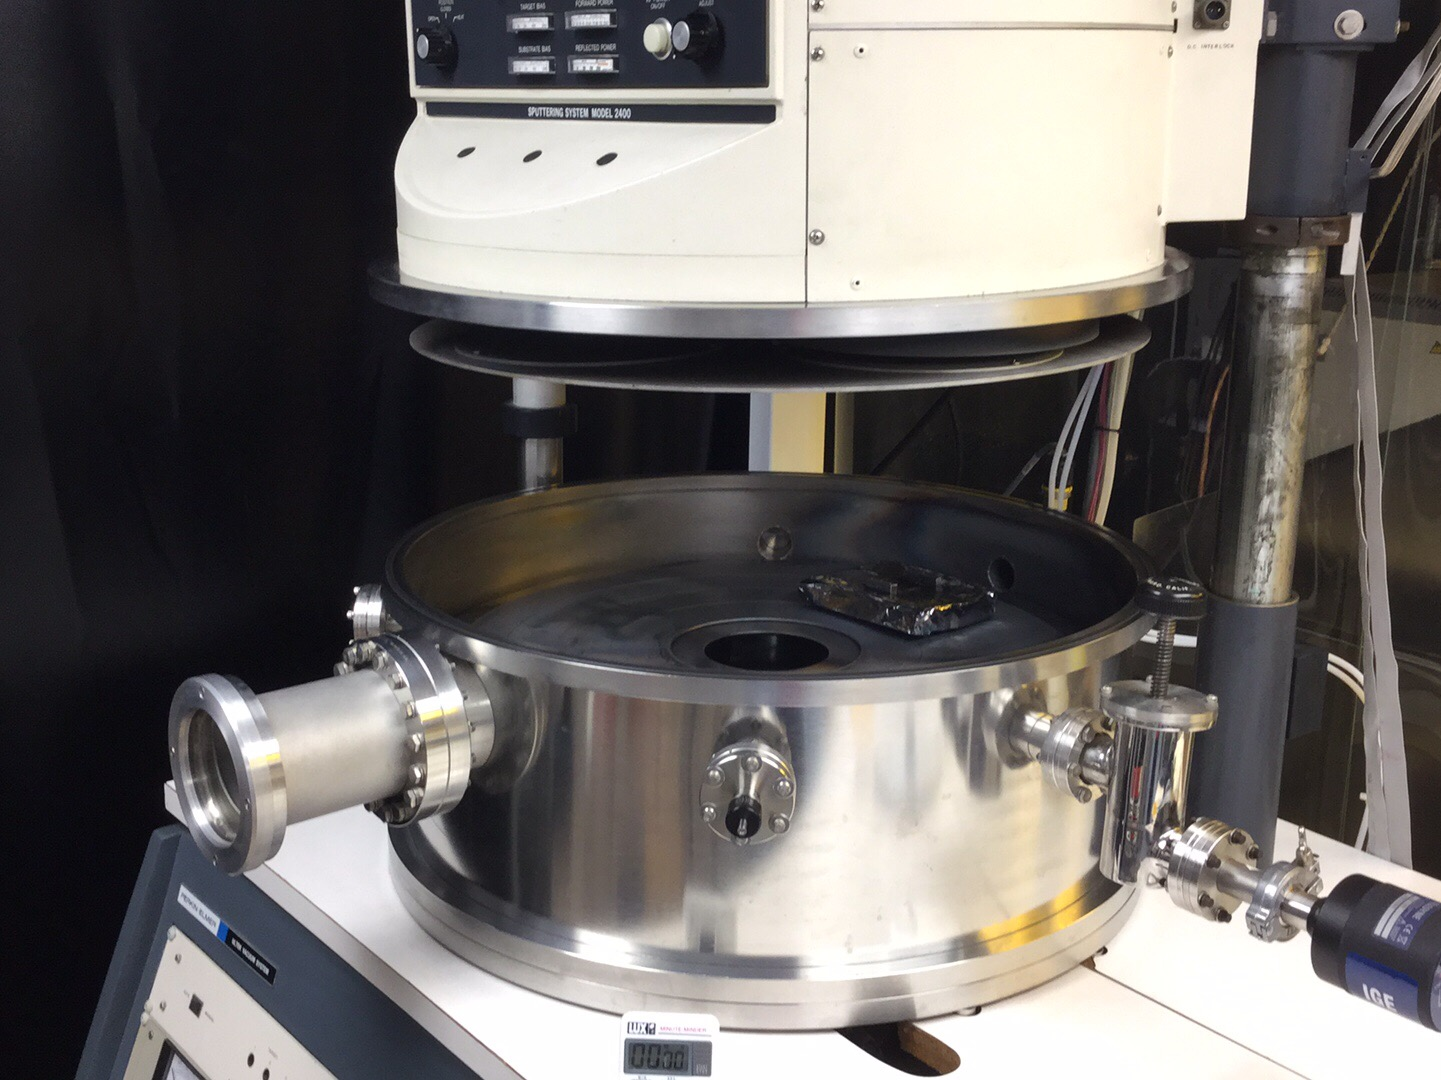
\includegraphics[width=0.6\textwidth]{sput-open.JPG}
\caption{Sputtering machine with chamber open}
\label{fig:sput-open}
\end{figure}
A jig is used to hold the detectors by the wings during the sputtering process.
It is designed to be adjustable, allowing for various detector sizes and geometries.
After the detector sample has been chemically etched it can be loaded onto the jig and then into the sputtering machine.

Once the sample is loaded the chamber can be closed and vacuum pumping can begin.
The first stage of pumping is done by a rough pump which takes the chamber from atmospheric pressure down to below 100 millitorr.
The rough pump is turned on or off by switching an electrical breaker located outside of the clean room.
After the pump is on and running normally, the roughing valve can be opened.
Opening the roughing valve allows the rough pump to vacuum the chamber from atmospheric pressure to around 100 mTorr.

Once the chamber has reached some pressure between 50-100 mTorr the roughing valve can be closed and the HY-VAC VALVE, shown as D in Figure \ref{fig:sput-flow}, can be opened.
The cryopump will then be able to vacuum the system to the required $10^{-6}$ Torr for sputtering.
The sputtering machine takes less than five minutes to go from atmosphere to $10^{-3}$ Torr using the rough pump and a further 2-3 hours to reach $10^{-6}$ Torr using the cryopump.

After proper vacuum pressure is achieved the sputtering deposition procedure can start.
The first thing is to start the water chiller and make sure the proper lines are selected.
The chiller is used to provide cooling to the target and stage during deposition as the plasma generates considerable heat.
It is located in the pump room and is show in Figure ~\ref{fig:water-cool}.
The middle picture of the figure shows the side view of the chiller where the separate lines to the sputtering and e-beam machines are visible.
The selection of lines is done by switching two valves on the back of the water chiller.
The handles of the valves indicate the direction of flow and is used to determine which line is selected.
\begin{figure}[htpb]
\centering
\includegraphics[width=\textwidth]{water-cool}
\caption{Water chiller for cooling the sputtering machine and e-beam evaporator}
\label{fig:water-cool}
\end{figure}

Once the water chiller has reached the set point temperature of \SI{10}{\celsius}, the deposition can start.
First the RF power supply should be turned on by flipping the switch at the base of the front.
The throttle valve, shown as C in Figure ~\ref{fig:sput-flow}, can now be turned on to limit the vacuuming of the chamber.
Now the mixed gas can be vented into the chamber using the gas flow adjuster show in the figure.
To the left of the flow controller is the togle switch to open the mixed gas line.
Then, the flow controller is turned on and set to approximately 50 SCCM.
Due to the throlle valve being on, the chamber will begin to increase in pressure based on the flow controller setting.
The key is to adjust the flow rate until a steady 14 mTorr chamber pressure is achieved.

After the chamber has stabalized at 14 mTorr the RF power can be introduced to the gas in order to generate the plasma required for sputtering.
This is done by pressing the power on button at the top of the chamber show in Figure.
The power can then slowly be increased to the marked point.
During this increase in power, the tune and load must be adjusted to keep the reflected power to a minimum and make sure all the power is transfed into the gas.
At a certain point, the plasma will form and the reading for forward and reflected power will jump up.
It is again necessary to quickly readjust the tune and load to get the reflected power back to 0.
After the reflected power is reduced, the power can be further adjusted to the required level, usually around 100 watts.
Once the plasma is generated, the user must wait for at least five minutes with the shutter closed to bombard the target and clean off the outer layer.
After this five minutes the shutter can be opened which will start deposition on the sample.
The machine can then be run for 15 minutes with the shutter open.
After 15 minutes have elapsed, the RF power can be turned off.
The detecor sample should have accumulated a layer of amorphous germanium that is around 300 nm thick.

The machine can then be opened up and the sample flipped over to coat the other side.
This is done by first turning down the flow rate of the mixed gas to zero and closing the valve.
Then the throttle valve can be turned off followed by closing the HY-VAC VALVE.
At this point the chamber should no longer be pumping so the vent valve can be opened and the chamber returned to atmospheric pressure.
The sample can then be flipped and the sputtering process starts again with closing the chamber and rough pumping.
\begin{sidewaysfigure}
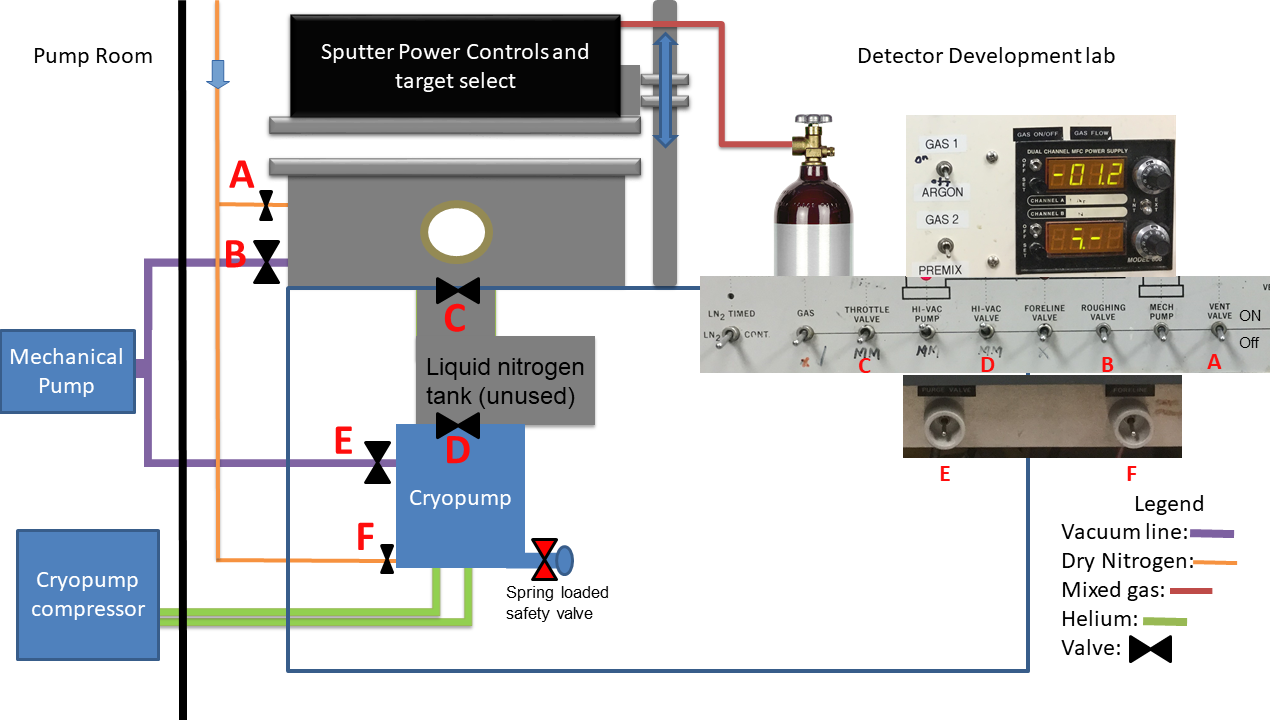
\includegraphics[width=\textwidth]{sput-flow}
\caption{This is a diagram of the Sputtering machine vacuum and gas system. Each valve is connected to a pressurized air line.}
\label{fig:sput-flow}
\end{sidewaysfigure}%}}}

% Section: Aluminum deposition%{{{
\section{Aluminum Deposition}
\subsection{Principles of e-beam}
\subsection{Operating Procedure}
Once the detector sample has been completely coated with a layer of amorphous germanium, aluminum can be deposited on the top and bottom surface to create the electrical contacts.
The aluminum serves as the electrical contact and covers the entire surface of the top and bottom which is what defines the detector as planar.

The e-beam has two separate power supplies: one for powering the controls and vacuum system, and another for supplying the high voltage to the electron gun.
To initiate the startup procedure, the control power supply is turned on.
Afterwords the controlls can be activated by switching the selector from 0 to 1 as seen in Figure \ref{fig:vac-control}.
This will supply power to the vacuum system which needs to be activated by following the prompts on the the screen.
Pressing start will initialize the system, activating the rough and turbo pump.
Once the turbo pump has reached 42 krpm it is ready to vacuum.
\begin{figure}[htpb]
\centering
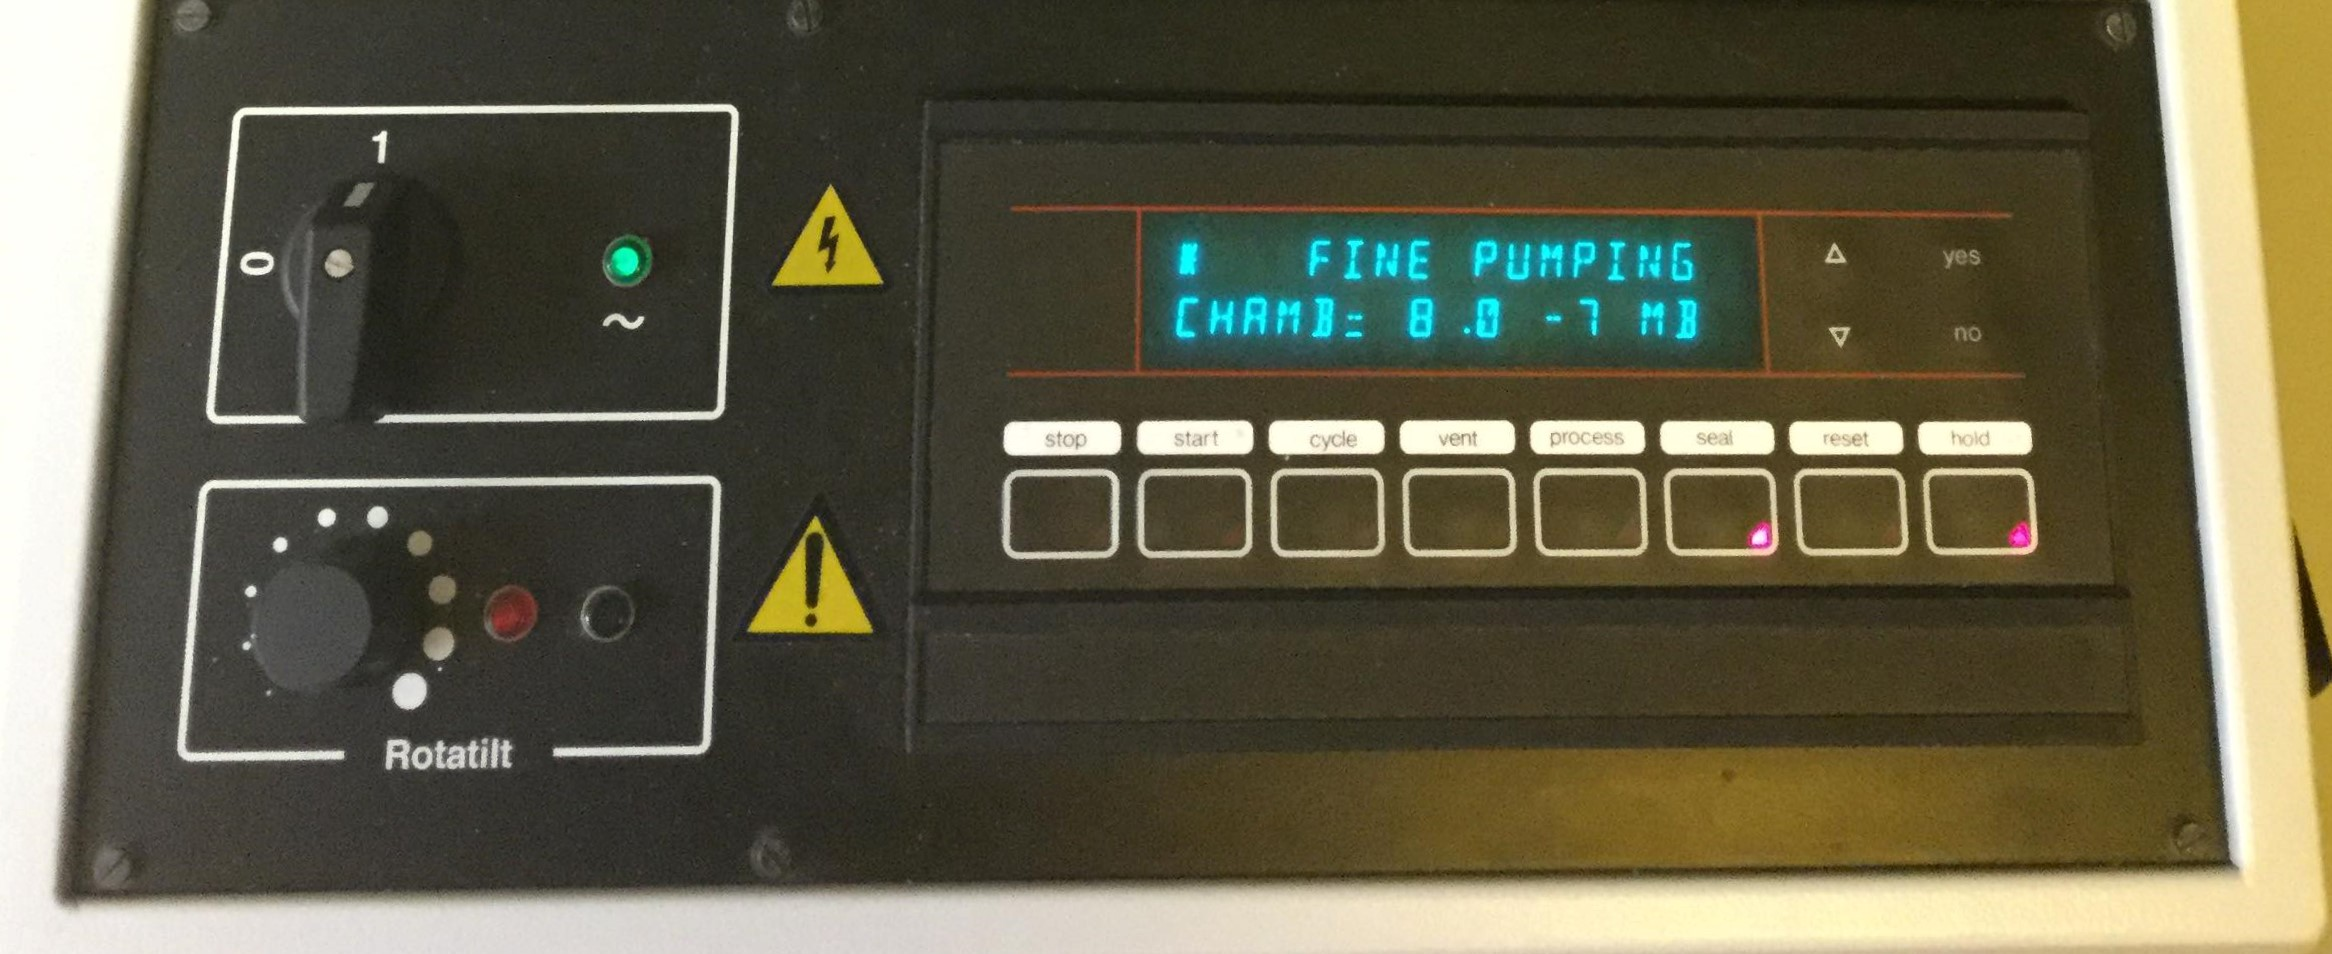
\includegraphics[width=\textwidth]{vac-control.JPG}
\caption{E-Beam vacuum controls and power switch}
\label{fig:vac-control}
\end{figure}

Pressing seal will isolate the turbo pump from the chamber and allow it to be vented so the sample can be placed inside.
Once sealed, the vent button can be pressed which will open the valve allowing nitrogen to fill the chamber.
After the chamber has reached atmospheric pressure the door will be able to open and the sample can be placed loaded onto the holder shown in Figure \ref{fig:ebeam-holder}
\begin{figure}[htpb]
\centering
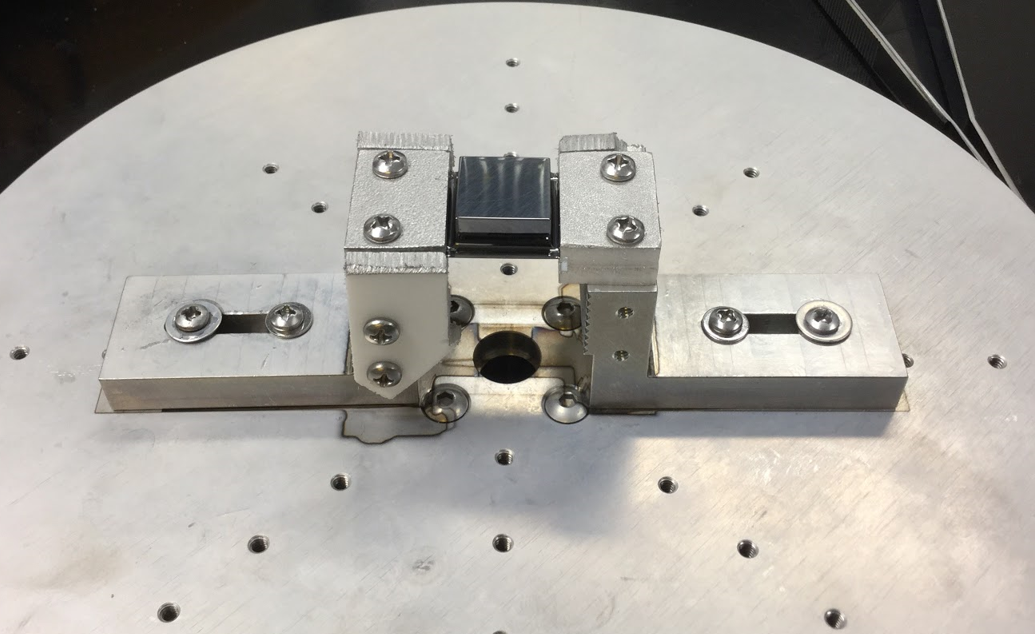
\includegraphics[width=0.6\textwidth]{ebeam-holder}
\caption{Sample holder for the E-Beam}
\label{fig:ebeam-holder}
\end{figure}

The e-beam, like the sputtering machine, is only operated under high vacuum.
The vacuum pumps are located in a cabinet directly under the e-beam chamber as shown in Figure \ref{fig:ebeam-flow}.

\begin{figure}[htpb]
\centering
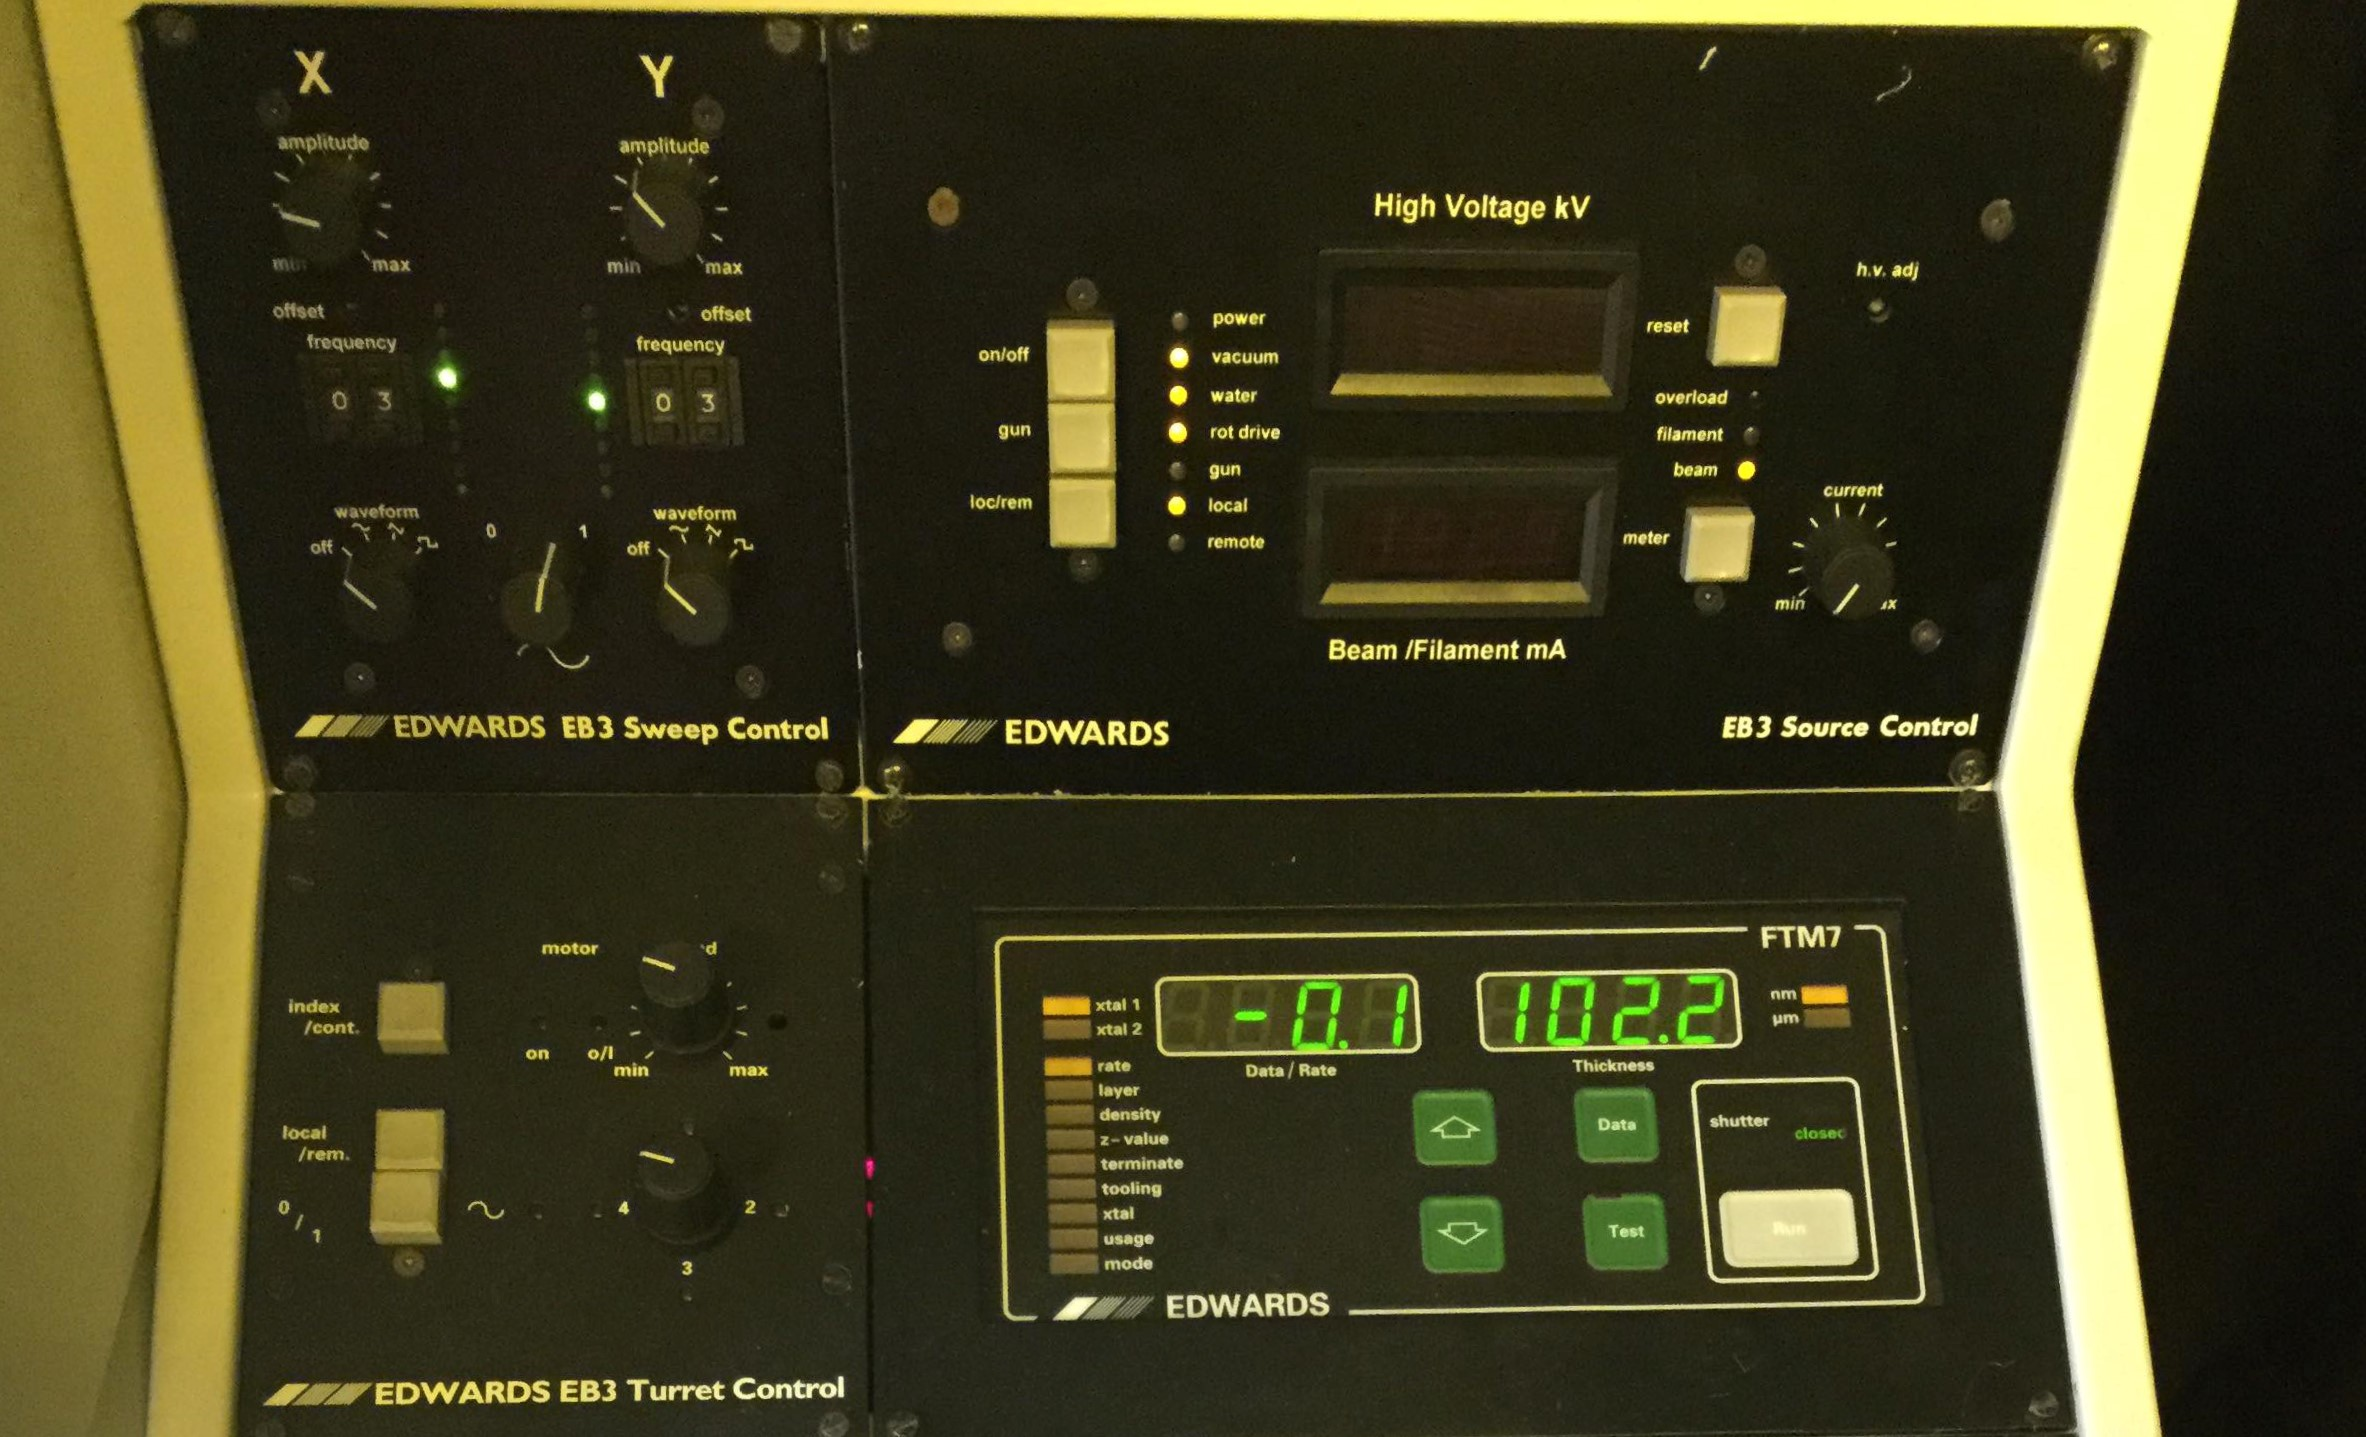
\includegraphics[width=\textwidth]{source-control.JPG}
\caption{E-Beam controls for the electron gun, sweep, crystal monitor, and crucible select}
\label{fig:source-control}
\end{figure}

\begin{sidewaysfigure}
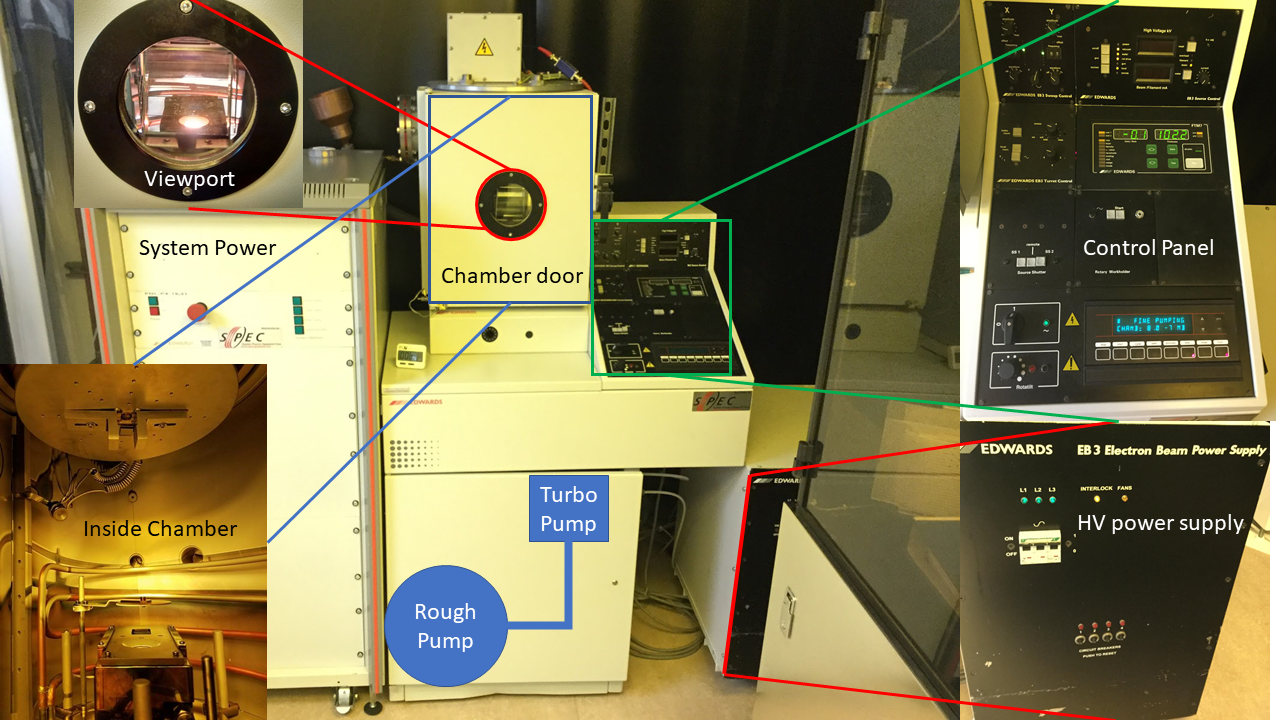
\includegraphics[width=\textwidth]{ebeam-flow}
\caption{This is a diagram of the of the electron beam machine.It is used to deposit aluminum onto the detector sample.}
\label{fig:ebeam-flow}
\end{sidewaysfigure}%}}}
% Section: Final Steps%{{{
\section{Final Steps}%}}}
